%!TEX root = ../paper.tex

\newcommand{\lightred}{red!75}
\newcommand{\lightblue}{blue!75}
\newcommand{\offset}{.1}

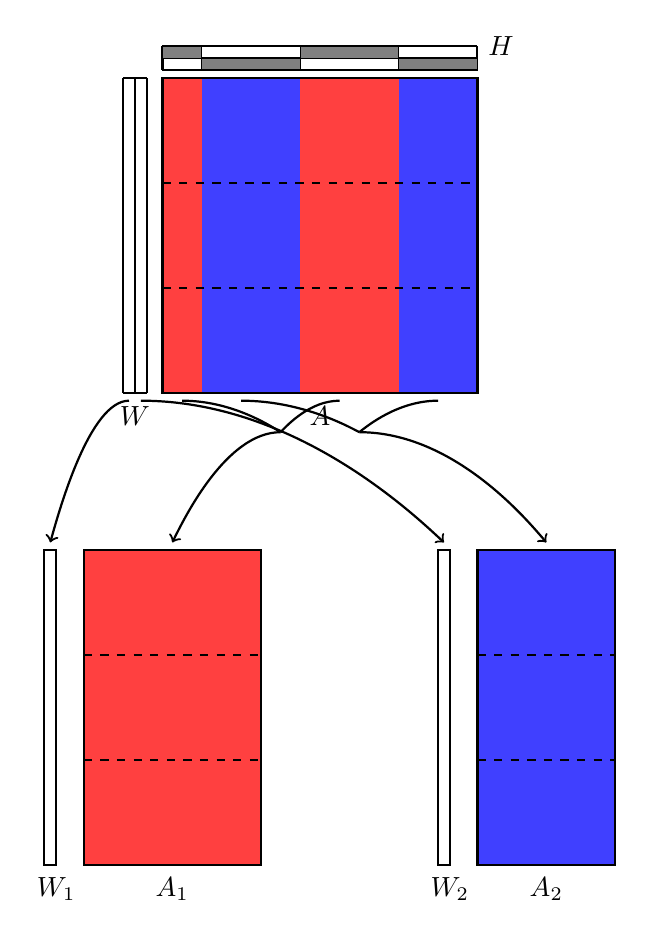
\begin{tikzpicture}

% draw A
\fill[\lightred] (0,0) rectangle ++(0.5,4);
\fill[\lightblue] (0.5,0) rectangle ++(1.25,4);
\fill[\lightred] (1.75,0) rectangle ++(1.25,4);
\fill[\lightblue] (3,0) rectangle ++(1,4);
\draw[thick,dashed,xscale=4,yscale=4/3] (0,0) grid ++(1,3);
\draw[thick] (0,0) rectangle (4,4);
\node at (2,-3*\offset) {$\M{A}$};

% draw W
\draw[thick,shift={(-.5,0)},xscale=.15,yscale=4] (0,0) grid ++(2,1);
\node at (-.5+.15,-3*\offset) {$\M{W}$};

% draw H
\draw[thick,shift={(0,4.1)},xscale=4,yscale=.15] (0,0) grid ++(1,2);
\node at (4+3*\offset,4.4) {$\M{H}$};
\draw[fill=gray,shift={(0,4.1)}] (0,.15) rectangle ++(.5,.15);
\draw[fill=gray,shift={(0,4.1)}] (.5,0) rectangle ++(1.25,.15);
\draw[fill=gray,shift={(0,4.1)}] (1.75,.15) rectangle ++(1.25,.15);
\draw[fill=gray,shift={(0,4.1)}] (3,0) rectangle ++(1,.15);

\begin{scope}[shift={(-1,-6)}]
	% draw A_1 and w_1
	\draw[thick,fill=\lightred] (0,0) rectangle ++(2.25,4);
	\draw[thick,dashed,xscale=2.25,yscale=4/3] (0,0) grid ++(1,3);
	\node at (1.125,-3*\offset) {$\M{A}_1$};
	\draw[thick] (-.5,0) rectangle ++(.15,4);
	\node at (-.5+.15,-3*\offset) {$\V{W}_1$};
	
	% draw A_2 and w_2
	\draw[thick,fill=\lightblue] (5,0) rectangle ++(1.75,4);
	\draw[thick,dashed,shift={(5,0)},xscale=1.75,yscale=4/3] (0,0) grid ++(1,3);
	\node at (5.875,-3*\offset) {$\M{A}_2$};
	\draw[thick,shift={(5,0)}] (-.5,0) rectangle ++(.15,4);
	\node at (5-.5+.15,-3*\offset) {$\V{W}_2$};
\end{scope}

% draw arrows to A_1 and w_1
% TODO: make these arrows prettier
\draw[thick] (0.25,-\offset) parabola (1.5,-0.5);
\draw[thick] (2.25,-\offset) parabola (1.5,-0.5);
\draw[thick,->] (1.5,-0.5) parabola (.125,-2+\offset);
\draw[thick,->] (-.5+.075,-\offset) parabola (-1.5+.075,-2+\offset);

% draw arrows to A_2
% TODO: make these arrows prettier
\draw[thick] (1,-\offset) parabola (2.5,-0.5);
\draw[thick] (3.5,-\offset) parabola (2.5,-0.5);
\draw[thick,->] (2.5,-0.5) parabola (4.875,-2+\offset);
\draw[thick,->] (-.5+.225,-\offset) parabola (3.5+.075,-2+\offset);

\end{tikzpicture}
